\documentclass[11pt]{article}

\usepackage[english,ngerman]{babel}
\usepackage{cite}
\usepackage{amsmath,amssymb,amsfonts} 
\usepackage{algorithmic}
\usepackage{graphicx}
\usepackage{textcomp}
\usepackage{xcolor}
\PassOptionsToPackage{hyphens}{url}\usepackage{url}
\usepackage{multicol}
\def\BibTeX{{\rm B\kern-.05em{\sc i\kern-.025em b}\kern-.08em
T\kern-.1667em\lower.7ex\hbox{E}\kern-.125emX}}

\author{
  	Jestram, Johannes\\
  	\texttt{jestram@posteo.de}
	\and
	Livert, Benedikt\\
	\texttt{benedikt.livert@gmx.de}
	\and
	Paranskij, Mark\\
	\texttt{mark.paranskij@gmail.com}
}

\title{Report Datenbankprojekt: Distributed Streaming EKF SLAM}

\begin{document}

\maketitle
\newpage

\tableofcontents
\newpage

\section{Einleitung}\label{Einleitung}
In verschiedenen technischen Disziplinen ist es nützlich, auf Grundlage des bisherigen Verhaltens eines Systems eine Voraussage über dessen künftigen Zustand treffen zu können. Ein Beispiel dafür ist die Navigation: Mithilfe der bisherigen Bewegungsrichtung und der aktuellen Geschwindigkeit lässt sich die Position des Objektes zu einem zukünftigen Zeitpunkt schätzen. Um eine möglichst verlässliche Vorhersage treffen zu können, müssen verschiedene Aspekte des betreffenden Systems gemessen werden. Da Messungen jedoch stets - in unterschiedlichem Maß - fehlerbehaftet sind, sollten diese Messfehler auch in die Betrachtung des Systemzustandes einbezogen werden. Weiterhin unterscheidet sich die Komplexität der Methoden zur Vorhersage des zukünftigen Zustandes je nach betrachtetem System. Möglicherweise wird der Zustandsübergang des Systems durch komplexe Funktionen mit vielen Parametern dargestellt. Zuletzt erscheint es auch als sinnvoll, die getroffene Vorhersage anhand neuer Messungen zu überprüfen und gegebenenfalls anzupassen. Eine Methode, um solche Zustandsübergänge vorherzusagen und zu überprüfen, ist der sogenannte Kal\-man Filter~\cite{kalman1960new}.

Ein weiteres, vor allem durch die moderne Robotik geprägtes, Problem ist das Kartographieren einer Umgebung. Zum einen muss der autonome Roboter stets seine eigene Position innerhalb der unbekannten Umgebung kennen, zum anderen soll er eben diese Umgebung erkunden und aufzeichnen. Die Erkundung der Umgebung basiert in der Regel auf der Messung mit eingebauten Sensoren, daher ist die Positionsbestimmung der Erkannten Objekte stets relativ zur eigenen Position. Andererseits verortet sich der messende Roboter innerhalb der soeben kartierten Umgebung. Die Genauigkeit der eigenen Positionsbestimmung und der erkundeten Objekte in der Umgebung hängen also in beide Richtungen unmittelbar zusammen. Beide Messungen unterliegen jedoch Fehlern, möglicherweise gibt es sogar Aussetzer bei der Erfassung der Sensordaten. Die Problemstellung erinnert an ein Henne-Ei Problem. Diese Problemstellung wird im englischen als ‘Simultaneous Localization and Mapping’ (SLAM) bezeichnet.

Es ist möglich, den Kalman Filter zur Lösung des  SLAM Problems zu nutzen~\cite{freiburg_SLAM}. Wie im Folgenden beschrieben werden wird, ist die Berechnung der Vorhersagen und deren Vergleiche mit den Messungen ein rech\-en\-auf\-wän\-di\-ger Algorithmus.

\subsection{Motivation}
In diesem Projekt wird als Datengrundlage der Victoria Park Datensatz betrachtet. Diesem Datensatz liegt die Bewegung eines Fahrzeugs durch besagten Park zugrunde. Der Zustand des Fahrzeugs wird durch eingebaute Sensoren sowie GPS regelmäßig gemessen. Darüber hinaus ermittelt das Fahrzeug mittels eines Lasersensors vor ihm liegende Objekte.

Basierend auf diesen Messungen soll der EKF/SLAM Algorithmus implementiert werden. Da die reine Implementierung des Verfahrens basierend auf dem gegebenen Datensatz bereits erfolgt ist~\cite{ute_SLAM}, wird es im Rahmen dieses Projektes darum gehen, wie ein solche Algorithmus parallelisiert werden kann. Um das EKF-SLAM Verfahren skalierbar zu machen, ist es folglich interessant dafür notwendigen Berechnungen zu parallelisieren. Es gilt zum Einen darum zu analysieren, inwiefern die Berechnungen selbst parallelisierbar sind. Weiterhin sind in den Anwendungsgebieten des Kalman Filter auch Szenarien denkbar, in denen Daten von mehr als einem System (z.B. Fahrzeug) verarbeitet werden sollen~\cite{vessel}. Für solche Szenarien stellt sich die Frage, ob  und wie Daten von mehreren Fahrzeugen möglichst effektiv verarbeitet werden können.

Dieses Projekt zielt folglich darauf ab, die parallele Implementierung des EKF SLAM Algorithmus umzusetzen und zu evaluieren. Dabei wird die Software für parallele und verteilte Verarbeitung von Datenströmen Apache Flink\footnote{\url{https://flink.apache.org/}} eingesetzt.

\subsection{Extended Kalman Filter}
Der Kalman Filter wurde im Jahr 1960 von Rudolph E. Kalman im Rahmen seines Papers “A New Approach to Linear Filtering and Prediction Problems”~\cite{kalman1960new} vorgestellt. Er ist ein Ansatz um Zustände zu schätzen. Der Kalman Filter minimiert die geschätzte Fehlervarianz. Der grundlegende Algorithmus funktioniert wie folgt~[Abb.~\ref{EKF-Algorithmus}]: Zunächst wird im sog. Prediction-Step der Zustand eines Systems zu einem Zeitpunkt $t$ auf Grundlage vorhergegangener Zustandsmessungen und einer Zustandsübergangsfunktion geschätzt. Diese Schätzung wird dann im Update-step (auch Correction-Step) nach dem Erhalt neuer Messdaten korrigiert und der Algorithmus beginnt von vorne.

\begin{figure}[!t]
	\centering
	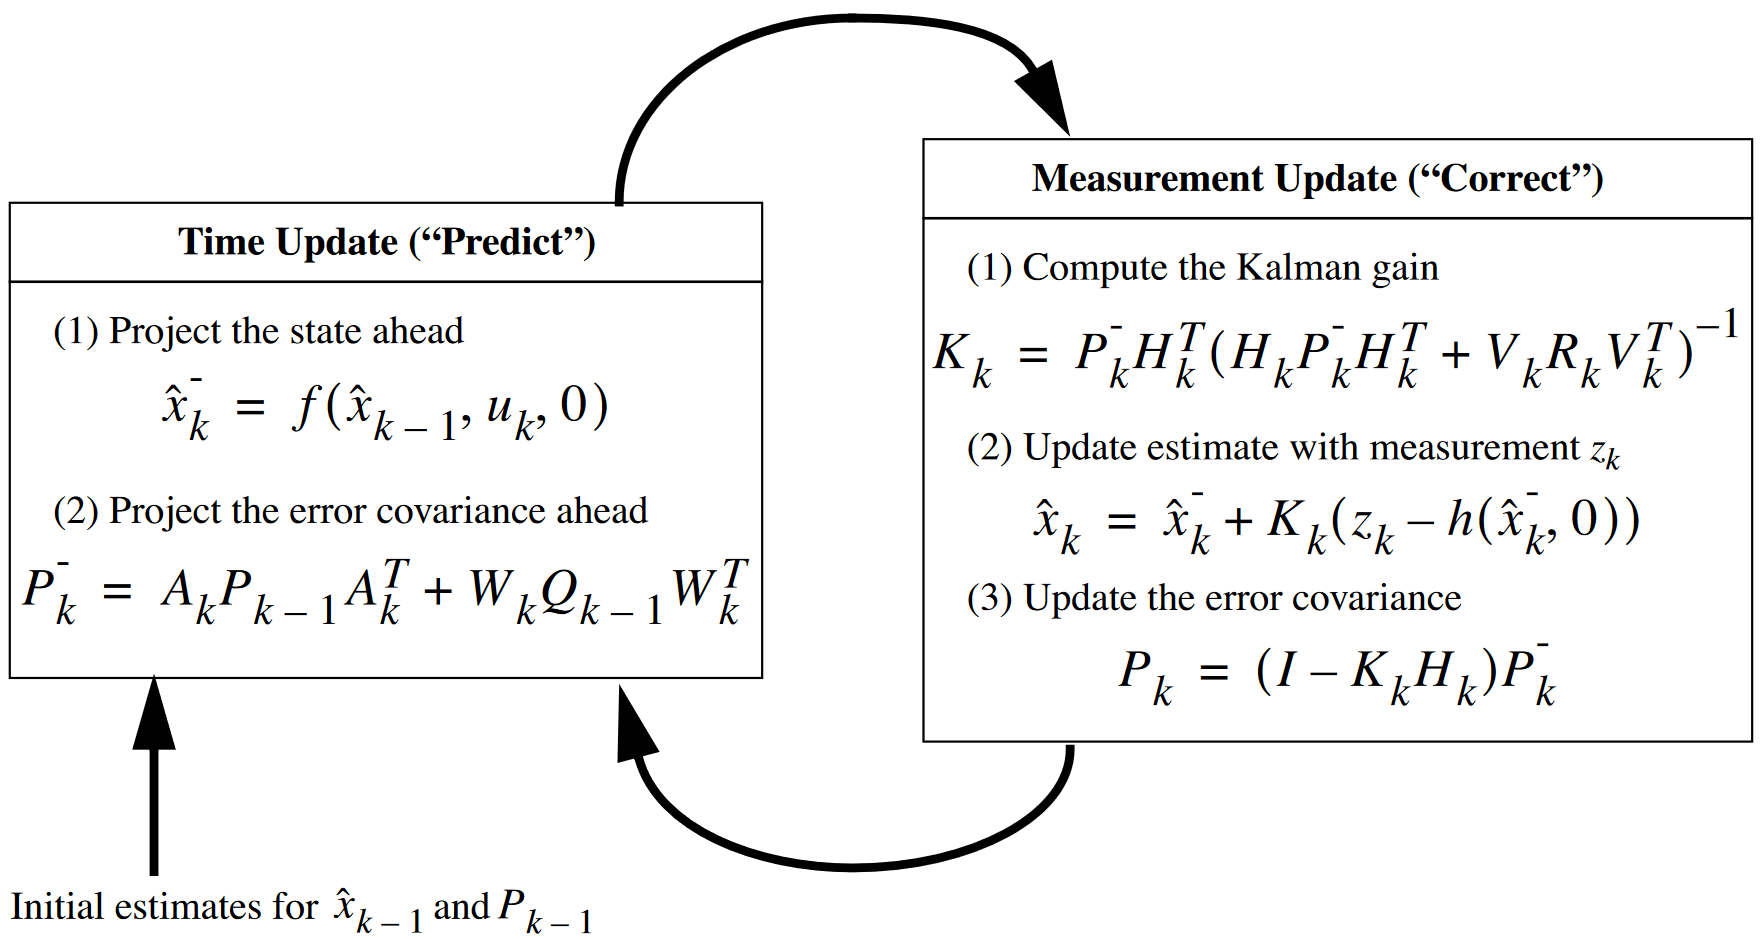
\includegraphics[width=5in]{EKF_algorithm.png}
	\caption{Extended Kalman Filter Algorithmus~\cite{EKF_course}.}
	\label{EKF-Algorithmus}
\end{figure}

Eine attraktive Eigenschaft dieses Algorithmus ist seine rekursive Natur; zur Berechnung des geschätzten neuen Zustands sind nur die Daten der vorherigen Messung nötig, da sich  in dieser alle vorherigen Messungen zusammengefasst wiederfinden. Der Extended Kalman Filter unterscheidet sich vom Diskreten Kalman Filter darin, dass die Zustandsübergänge durch nichtlineare Funktionen abgebildet werden. Die Nichtlinearität verkompliziert den Algorithmus, wie im folgenden gezeigt wird.

\subsubsection{Prediction-Step}
Der Zustand eines Systems kann über beliebig viele Parameter dargestellt werden. Um einen Zustand $\hat{x}_t$ in einen Zustand $\hat{x}_{t+1}$ zu überführen, muss für jeden Parameter eine Funktion definiert werden, die diesen Übergang abbildet. Im falle eines Fahrzeuges erfolgt dies über die Erstellung eines Bewegungsmodells. Auf Grundlage der Sensorik und vorhandenen Messwerte muss das Bewegungsmodells den Zustand, korrekt und dargestellt in die gewünschten Metriken, berechnen.

Doch das Bewegungsmodell ist nicht der einzige Einflussfaktor für den Zustandsübergang: Messfehler und äußere Einflussfaktoren sorgen für Ungenauigkeiten. Diese Ungenauigkeiten werden im Extended Kalman Filter berücksichtigt, wie im folgenden erläutert wird.

\subsubsection{Update-Step}
Der im Prediciton-Step geschätzte Zustand wird nun basierend auf neuen, externen Beobachtungen des Zustandes korrigiert. Jedoch ist es nicht so, dass die Schätzung einfach auf die äußere Beobachtung gesetzt wird. Die Korrektur wird gedämpft um den sog. Kalman Gain. Dieser berechnet sich sowohl aus Messunsicherheiten, als auch eine Kovarianzmatrix, die die Abhängigkeiten zwischen den einzelnen Parametern des Zustands abbildet. WARUM LINEARISIERUNG Weiterhin muss das nichtlineare 

\subsection{Simultaneous Localization and Mapping}

\section{Methodik}\label{Methodik}
\subsection{Verwendete Software}
Im folgenden werden zunächst die dem Projekt zugrunde liegenden Konzepte detailliert vorgestellt. Danach wird erklärt, welche softwareseitigen Werk\-zeu\-ge zur Umsetzung benutzt werden und warum. An dieser Stelle wird der Fokus auf den für das Projekt relevanten Funktionalitäten der jeweiligen Software liegen. Anschließend werden wir ausführlich auf die bereitgestellten Daten eingehen und deren Spezifika erläutern, da dieses Wissen Grundlage der Implementierung des Algorithmus ist. Als nächstes werden wir ausgewählte Designentscheidungen der Implementierung vorstellen. Die Ergebnisse bzw. die Ausgabe unserer Implementierung werden im Anschluss dokumentiert, analysiert und bewertet.

\subsubsection{Apache Flink}
Flink ist eine Software zur verteilten und parallelen Verarbeitung von Stream- oder Batch\-daten. Es ist aus dem Stratosphere Projekt\footnote{\url{http://stratosphere.eu}}~\cite{alexandrov_stratosphere_2014} der TU-Berlin hervorgegangen und ein Top-Level-Projekt der Apache Foundation \footnote{\url{https://apache.org}}. Die Software ist per Open Source Lizenz verfügbar und aufgrund der hohen Performanz~\cite{alexandrov_stratosphere_2014} ein beliebtes Werkzeug für verteilte und skalierbare Datenverarbeitung.

\begin{figure}[!t]
	\centering
	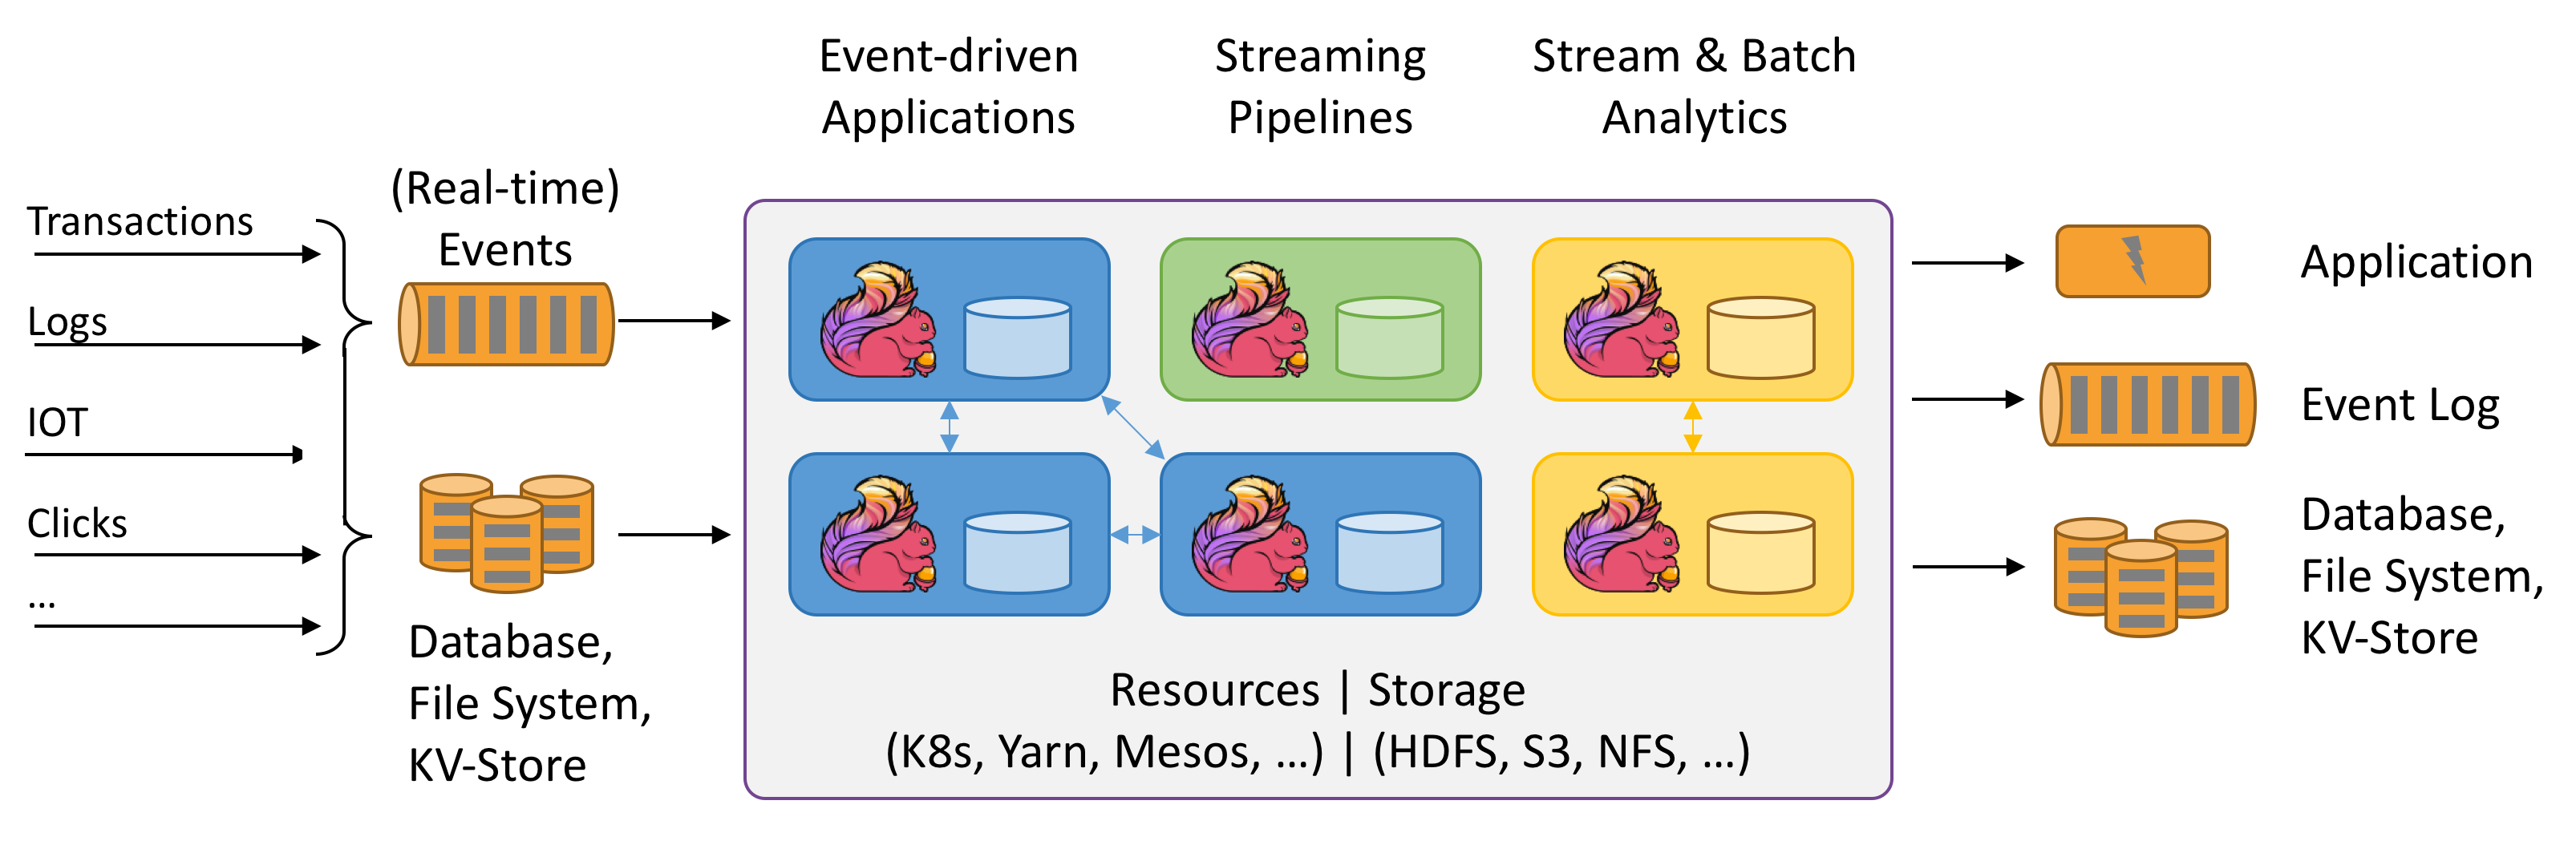
\includegraphics[width=5.5in]{flink-home-graphic.png}
	\caption{Überblick über die Funktionen von Apache Flink~\cite{Flink-Overview-Link}.}
	\label{Flink-Überblick}
\end{figure}

\begin{figure}[!t]
	\centering
	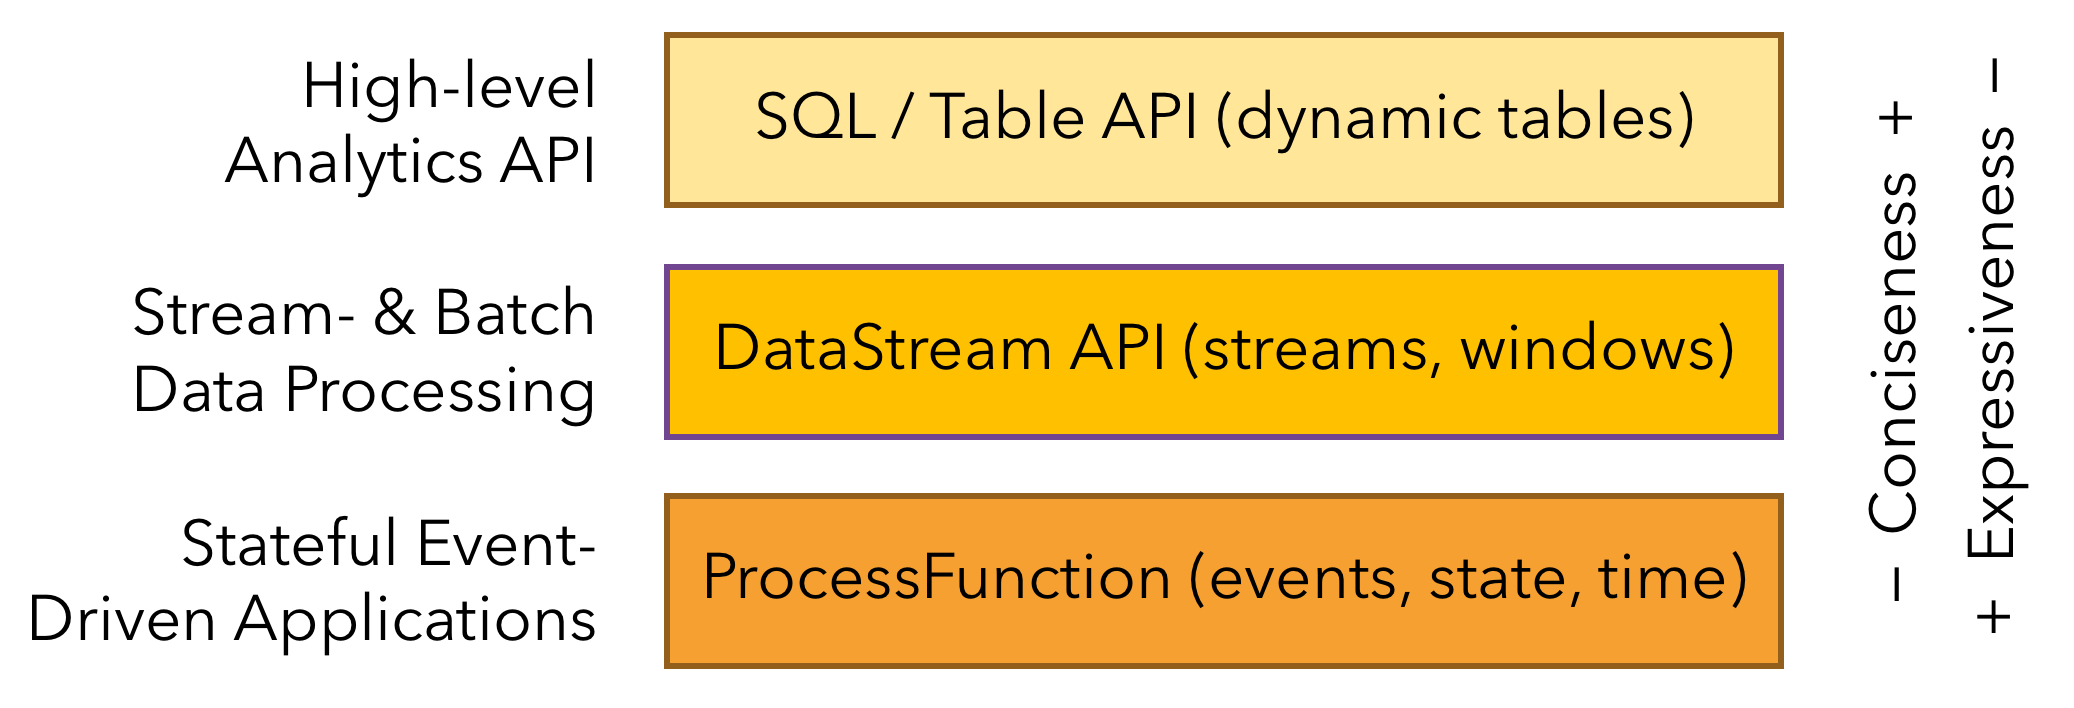
\includegraphics[width=4in]{Flink-api-stack.png}
	\caption{APIs auf verschiedenen Abstraktionsniveaus~\cite{Flink-APIs-Link}.}
	\label{Flink-APIs}
\end{figure}

Flink basiert auf der Java Virtual Machine (JVM) und ist in Scala und Java implementiert~\footnote{\url{https://github.com/apache/flink}}. Der Funktionsumfang umfasst die parallele und verteilte Verarbeitung von Datenströmen, sowie einmaligen (in der Regel sehr rechenaufwändigen) sog. Batch-Aufträgen~[Abb.~\ref{Flink-APIs}]. Dazu stehen verschiedene Application Programming Interfaces (APIs) auf unterschiedlichen Abstraktionsebenen zur Verfügung~[Abb.~\ref{Flink-Überblick}].

Da das Ziel dieses Projektes die Anwendung von EKF-SLAM auf mehrere Fahrzeuge in Echtzeit ist, wird vor allem die DataStream API genutzt. Diese liefert vorgefertigte Funktionalitäten für viele übliche Aufgaben in der Verarbeitung von Datenströmen. Diese umfassen unter anderem die automatisierte parallelisierung der Verarbeitung von Datenströmen. Weiterhin ist es möglich, eingehende Daten mit sog. Schlüsseln (engl. keys) zu versehen und die weitere Verarbeitung der Daten im Folgenden abhängig von dem zugeordneten Key zu mache. Dies erfolgt über die Klassen KeyedDataStream und KeyedDataPoint. Ein KeyedDataStream verarbeitet generische Datentupel, welche jeweils mit einem Zeitstempel und einem Schlüssel versehen sind. Dabei liefern KeyedDataPoint eine Art Blaupause für den Inhalt eines einzelnen Datentupels.

Mit Hilfe solcher geschlüsselter Datenströme ist es möglich, für jeden Schlüssel einen eigenen Zustand (engl. state) zu definieren. Folglich ist es mit Schlüsseln und Status möglich, Daten und darauf basierende Berechnungen nach deren Quelle oder Zugehörigkeit klar voneinander zu trennen.

\subsubsection{InfluxDB}
InfluxDB\footnote{\url{https://www.influxdata.com/products/influxdb-overview}} ist eine für Zeitreihendaten optimierte Datenbank. Die Interaktion erfolgt in einer Anfragesprache ähnlich zu SQL. Es existieren APIs für verschiedene Programmiersprachen, unter anderem Java. 

Jedes zu speichernde Datentupel muss mit einem Zeitstempel versehen sein. Wie in Flink ist auch hier möglich, eingehende Daten anhand eines Schlüssels zu unterscheiden. Daten können in unterschiedliche Datenbanken gespeichert werden und innerhalb einer Datenbank nach Messreihen unterschieden werden. Einzelne Messungen werden in sog. Feldern gespeichert. Anzahl und Typ des Inhalts der einzelnen Felder können durch den Nutzer festgelegt werden. Dank der genannten Funktionen bietet InfluxDB eine leistungsfähige Lösung für die anwendungsspezifische Speicherung von Echtzeitdaten.

\subsubsection{Colt}
Zur Implementierung des Extended Kalman Filter benötigt man in Java eine externe Library, da Java in der Version 1.8, die wir verwendet haben, keine native Möglichkeit bereitstellt auf Matrizen und Vektoren, anders als in Form von Listen oder Arrays, zu arbeiten. Somit haben wir uns für die Colt 1.2 Library~\footnote{\url{https://dst.lbl.gov/ACSSoftware/colt}} entschieden, welche am CERN entwickelt wurde, da alle für uns notwendigen Matrix- und Vektoroperationen durch Colt zur Verfügung gestellt werden.

\subsection{Victoria Park Datensatz}
Die Inhalte dieses Datensatzes \footnote{\url{https://www.mrpt.org/Dataset_The_Victoria_Park}} wurden im Jahr 2006 im Victoria Park in Sydney gesammelt. Es wurde die Bewegung eines Fahrzeugs durch den Park aufgezeichnet und währenddessen vom Fahrzeug Objekte in der nahen Umgebung erfasst. Die Dauer der Aufzeichnungen ist rund 25 Minuten.

\subsubsection{Messungen}
Es existieren drei verschieden Quellen für Messungen. Die internen Sensordaten liefern die Odometrie. Diese setzt sich aus dem Lenkwinkel \(\alpha\), sowie der Geschwindigkeit \textit{v}, gemessen am linken Hinterrad, zusammen. Außerdem wurde regelmäßig die Position des Fahrzeuges via GPS bestimmt. Die Messung der in der Umgebung befindlichen Objekte erfolgt mittels eines Lasersensors.

Neben den rohen Messungen existieren unterschiedlich aufgearbeitete Datensätze. Diese unterscheiden sich in der Anzahl der enthaltenen Datenpunkte sowie der Formatierung der Werte. Die Odometriedaten werden stets gemeinsam im Format {Zeitstempel, Lenkwinkel, Geschwindigkeit} angegeben. Es existiert eine Datei mit rund 66.000 Messungen und eine mit rund 4.000.

Auch die GPS-Daten werden in mehreren Versionen geliefert. Generell ist festzustellen, dass die GPS-Messungen in regelmäßigen Abständen von 200ms geliefert werden. Jedoch sind teils starke zeitliche Lücken in den Messungen vorhanden, sodass über einen längeren Zeitraum keine Positionsbestimmung erfolgt. Auch enthält der Datensatz einige Ausreißer. Diese erkennt man daran, dass das Auto, falls diese Messungen korrekt wären, von einem zum nächsten Punkt eine viel zu große Distanz zurücklegen würde. Beide genannten Mängel wurden auch von den Autoren des Datensatzes erkannt und benannt.

Der Lasersensor ist über der vorderen Stoßstange des Fahrzeugs positioniert und vermisst einen 180-Grad Winkel. Dieser Blickwinkel ist wird mit 361 Messpunkten von rechts nach links (in Fahrtrichtung) abgetastet. Für jeden einzelnen Messpunkt speichert der Laser den Abstand des gemessenen Objektes. Die Messungen sind für Objekte, die sich höchstens 80m entfernt befinden, hinreichend präzise. 

\subsubsection{Probleme mit den Daten}
Im Laufe des Projektes stellte sich der Umgang mit den Daten als das zeitaufwändigste Problem dar. Vor allem die unterschiedlichen Versionen desselben Datensatzes sorgten für regelmäßige Probleme.

Auf der Website des Datensatzes~\footnote{\url{https://www.mrpt.org/Dataset_The_Victoria_Park}} befindet sich ein Datensatz bestehend aus 4832 Datenpunkten, der laut Dokumentation mit hilfe eines externen Tools, des Rawlog Viewers~\footnote{\url{https://www.mrpt.org/list-of-mrpt-apps/rawlogviewer}}, als Textdatei extrahiert und visualisiert werden kann. Diese 4832 Datenpunkte setzen sich zur Hälfte aus Inkrementen zwischen zwei Messungen in Richtung der X-Achse, Y-Achse und der Drehung des Fahrzeuges zusammen, sowie 2416 Lasermessungen. Problematisch bei diesem Datensatz ist hierbei jedoch die Tatsache, dass die komplexe Geometrie zwischen Geschwindigkeitsmessung und Laser- und GPS-Messung am Fahrzeug nicht näher dokumentiert war, was zu einem hohen Maß an Ambiguität bezüglich der Verarbeitung des Datensatzes geführt hat. 

Darüber hinaus befindet sich auf der originalen Seite für den Datensatz der Publikation~\footnote{\url{http://www-personal.acfr.usyd.edu.au/nebot/victoria_park.htm}} ein Datensatz im ASCII Format. Dieser ist aus 69941 Datenpunkten zusammengesetzt, von denen 61763 Odometrie Daten sind, die jeweils einen Zeitstempel, die Geschwindigkeit in Metern pro Sekunde und den Winkel der Vorderachse des Fahrzeuges beinhalten. Dazu kommen 948 Datenpunkte für GPS-Messungen, sowie 7230 Lasermessungen.

Ebenfalls, befindet im originalen Download~\footnote{\url{https://www.mrpt.org/Dataset_The_Victoria_Park}} ein MatLab Datensatz, den wir mit Hilfe eines Python-Skriptes ausgelesen haben, welcher sich aus 61945 gleich zusammengesetzten Odometrie Datenpunkten, 4466 GPS-Messungen und 7249 Lasermessungen, insgesamt also 73660 Datenpunkten, ergibt.

Aufgrund eines Mangels an definitiver Information und inkohärenter Datensätze wurde der Projektfortschritt lange durch das auswerten dieser Datensätze hinausgezögert. Hierbei haben wir versucht durch die Visualisierung der Daten diese zu validieren. Dies war führte bei dem kleinen Datensatz, bestehend aus 4832 Datenpunkten, zu keinem Erfolg, da das Format der Inkremente nicht ausreichend dokumentiert ist, und wir erst mit viel Recherche und durch interne Informationen aus dem Rawlog Viewer~\footnote{\url{https://www.mrpt.org/list-of-mrpt-apps/rawlogviewer}} auf das zugrundliegende Bewegungsmodel des Datensatzes~\footnote{\url{https://www.mrpt.org/tutorials/programming/odometry-and-motion-models/probabilistic_motion_models}} gestoßen sind.

In visualisierter Form waren lediglich die GPS-Messungen des MatLab Datensatzes ähnlich der Form des bekannten Victoria Parks, wodurch wir uns entschlossen haben EKF aus Basis der GPS Daten auf diesem Datensatz anzuwenden um das Projekt voranzutreiben.
Gesamtheitlich betrachtet machten die genannten Probleme mit dem Datensatz circa die Hälfte der Projektarbeit aus. Selbst am Ende des Projektes kam es noch dazu, dass wir verschiedene Eingangsdaten ausprobieren mussten, um valide und funktionierende Ergebnisse zu erzielen, da beispielsweise der ASCII Datensatz gravierend vom MatLab Datensatz abweicht und aus unserer Perspektive als falsch anzusehen ist. So weichen die GPS-Messungen der beiden Datensätze gänzlich voneinander ab und die Odometrie durch den gleichen EKF-Algorithmus verarbeitet, resultiert in komplett unterschiedlichen Ergebnissen.

\subsubsection{Ausreißer}
Wie bereits aus der Quelle für den Datensatz (viktoria park paper reference) hervorgeht, sind die GPS-Messungen fehlerhaft und unvollständig und wurden daher nicht weiter verwendet. Da es aufgrund der unterschiedlichen Datensätze notwendig wurde den EKF in der einfachsten Form mit GPS zu implementieren, mussten wir dennoch auf den Datensatz zurückgreifen. Damit es trotzdem vergleichbare und repräsentative Ergebnis für den EKF mit GPS geben konnte, entschieden wir uns dazu den GPS Datensatz um Ausreißer basierend auf einer Heuristik zu bereinigen. Hierbei werden Datenpunkte die eine zu hohe Distanz zu vorherigen GPS Messungen aufweisen, sowie in kleinen Gruppen von wenigen Tupeln vorkommen aussortiert. Dabei waren bereits mit 21 Tupeln weniger die signifikantesten Ausreißer beseitigt.

\subsection{Implementierung}

\subsubsection{Simulatiaon mehrerer Fahrzeuge}
Da es in diesem Projekt auch um die Parallelisierung der Verarbeitung von Daten unterschiedlicher Fahrzeuge geht, haben wir den vorhandenen Datensatz mehrfach repliziert. So kann die Berechnung mehrerer Systeme und deren Zustände simuliert und mit Hilfe von Flink parallelisiert werden. Die replizierten Daten haben wir zur besseren Veranschaulichung verändert; beispielsweise wurde die Reihenfolge der Tupel umgekehrt oder nur Teile des vollständigen Datensatzes für unterschiedliche simulierte Fahrzeuge verwendet.

\subsubsection{Umsetzung in Apache Flink}
Apache Flink unterscheidet Arbeitsaufträge in Streaming- und Batch-Auf\-trä\-ge. Diese unterscheiden sich in der Art und Weise der Parallelisierung der Berechnungen: bei Streams müssen beispielsweise Aggregationen mit einem Fenster versehen werden, da man sie bei einem potentiell unendlich langen Datenstrom nicht auf die gesamten Daten ausführen kann. Bei Batch-Daten ist das im Gegensatz möglich.

Da die Nutzung des Kalman Filters vor allem vor dem Hintergrund von kontinuierlich, über einen langen Zeitraum eintreffenden Datenströmen sinnvoll ist, fiel die Entscheidung auf einen Streaming-Auftrag.

In Apache Flink ist sowohl die EKF auf Basis von GPS Daten, als auch die Implementierung der EKF-SLAM Algorithmus als eine Map-Funktion umgesetzt. Dies bedeutet, dass die Funktion ein Tupel nach dem anderen übergeben bekommt, was die Problematik mit sich bringt, die Tupel des Prediction-Step und die Tupel des Update-Step zu unterscheiden, als auch vorhergegangene Rückgabewerte die zur Berechnung des neuen Zustandes notwendig sind zu persistieren. Die erste Problematik wurde gelöst indem jedem KeyedDataPoint ein Parameter beim Parsing übergeben. So bekommen beispielsweise Odometrie Datenpunkte den bezeichner “odo” hinzu. Das Problem der Persistierung zwischen einzelnen Map-Schritten, wird dadurch behandelt, dass ein Zustandsobjekt erzeugt wird, welches den vorherigen Zustand des Fahrzeuges als Vektor, sowie die Kovarianzmatrix, und den Zeitstempel des vorherigen Tupels beinhaltet um nachgelagerte Berechnungen zu ermöglichen.

Abgesehen von der Implementierung des EKF/SLAM Algorithmus bestand die Kernherausforderung beim Implementieren in der Parallelisierung der Berechnungen. Dazu mussten zum einen die Daten der unterschiedlichen Fahrzeuge auch bei der Verarbeitung dem entsprechenden Fahrzeug zugeordnet werden. Da jedes Fahrzeug einen eigenen, distinkten Zustand hat, dürfen die eingehenden Daten nicht vermischt werden. Zur Umsetzung dieser Unterscheidung dienten uns vor allem KeyedDataStreams. Jedes Fahrzeug verfügt über eine eigene ID. Diese ID wird dann zum Schlüssel des KeyedDataStreams, sodass die interne Zuordnung der Eingangsdaten eindeutig und korrekt ist. Die Berechnungen können durch die Schlüssel also für jedes Fahrzeug parallelisiert werden.

\subsubsection{EKF Implementierung}
\paragraph{Prediction Schritt und Bewegungsmodell}
Für den EKF ohne SLAM, der folglich eine GPS-Messung als Grundlage des Update-Step verwendet, initialisierten wir den Filter mit folgenden Werten und Funktionen:

Der Zustand des Fahrzeugs wird durch die x- und y-Koordinaten sowie den Winkel des Fahrzeuges zur x-Achse des Koordinatensystems angegeben.
\begin{equation}\label{EKF-State-Vector}
	\hat{x}_t = \begin{pmatrix}
		x_t \\
		y_t \\
		\phi_t \\
	  \end{pmatrix}
\end{equation}

Da sich der find the bug Sensor zur Geschwindigkeitsmessung am linken Hinterrad befindet, muss die Messung noch auf die Fahrzeugmitte zentriert werden.
\begin{equation}\label{Geschwindikeit}
\begin{split}
	v &= \frac{v_{Messung}}{1-\tan(\alpha)*\frac{H}{L}} \\
	&\text{mit } \\
	v &= \text{Fahrzeuggeschwindigkeit} \\
	v_{Messung} &= \text{Geschwindigkeit am linken Hinterrad} \\
	H &= \text{Achsabstand Sensor zur Fahrzeugmitte} = 0,76m \\
	L &= \text{Abstand Hinterachse zur Vorderache} = 2,83m
\end{split}
\end{equation}

Die Zustandsvorhersage $\hat{x}_{t+1}^-$ ergibt sich aus einem Bewegungsmodell, das anhand der vergangenen Zeit $\Delta T$ zwischen dem letzten Update- und dem jetzigen Prediction-Step die neue Position des Fahrzeuges schätzt. 
\begin{equation}\label{EKF-Motion-Model}
\begin{split}
	\hat{x}_{t+1}^- &= f(\hat{x}_{t},u_t) = \begin{pmatrix}
		x_{t+1} \\
		y_{t+1} \\
		\phi_{t+1} \\
	  \end{pmatrix} \\
	  &= \begin{pmatrix}
		  x_{t}+\Delta T(v\cos(\phi_t)-\frac{v}{L}\tan(\alpha))*(a\sin(\phi_t)+b\cos(\phi_t)) \\
		  x_{t}+\Delta T(v\sin(\phi_t)+\frac{v}{L}\tan(\alpha))*(a\cos(\phi_t)-b\sin(\phi_t)) \\
		  \phi_t + \Delta(\frac{v}{L}\tan(\alpha)) \\
	  \end{pmatrix}
\end{split}
\end{equation}

Während des EKF wird die Kovarianzmatrix $P$ in jedem Durchlauf verändert. Wir initialisieren sie mit einem hohen Wert, sodass sie sich innerhalb der ersten Durchläufe stark verändert. 
\begin{equation}\label{EKF-Initiale-Kovarianzmatrix}
	P_{0} = \begin{pmatrix}
		0 & 0 & 0 \\
		0 & 0 & 0 \\
		0 & 0 & 0 \\
	  \end{pmatrix}
\end{equation}

Für die Linearisierung des Bewegungsmodells, i.e. zur Aktualisierung von $P$, im EKF wird außerdem noch die Jakobi-Matrix des Bewegungsmodells benötigt.
\begin{equation}\label{EKF-Motion-Model-Jakobi-Matrix}
\begin{split}
	F_{ekf} &= \frac{\partial f}{\partial \hat{x}} \\
	&= \begin{pmatrix}
		1 & 0 & -\Delta T(v\sin(\phi_t)+\frac{v}{L}\tan(\alpha)*a\cos(\phi_t)-b\sin(\phi_t)) \\
		0 & 1 & \Delta T(v\cos(\phi_t)-\frac{v}{L}\tan(\alpha)*a\sin(\phi_t)+b\cos(\phi_t)) \\
		0 & 0 & 1 \\
	  \end{pmatrix}
\end{split}
\end{equation}

\paragraph{Update Schritt}
Im Update Schritt werden die Ergebnisse des Prediction Schritt mit Hilfe der GPS-Messung aktualisiert. Dazu muss zunächst das Beobachtungsmodell definiert werden; dessen Aufgabe ist es, die Messungen des GPS-Sensors auf das Format des Zustandsvektors abzubilden. Im vorliegenden Fall werden x- und y-Koordinate im passenden Format gemssen. Der Winkel $\phi$ wird durch den GPS-Sensor nicht gemessen und daher auch nicht im Beobachtsungsmodell abgebildet. Der auf Grundlage des Beobachtungsmodells berechnete Kalman Gain $K_t$ wird aufgrund seiner Dimensionalität dennoch $\phi$ beeinflussen.
\begin{equation}\label{EKF-Observation-Model}
	z_{ekf} = h(\hat{x}) = \begin{pmatrix}
		x_{gps} \\
		y_{gps} \\
	\end{pmatrix}
\end{equation}

Zwar ist das Beobachtungsmodell linear, da jedoch aufgrund des nichtlinearen Bewegungsmodells der Extended Kalman Filter verwendet wird, muss auch vom Beobachtungsmodell die Jakobi-Matrix gebildet werden.
\begin{equation}\label{EKF-Observation-Model-Jakobi-Matrix}
	H(\hat{x})= \frac{\partial h}{\partial \hat{x}} = \begin{pmatrix}
		1 & 0 & 0 \\
		0 & 1 & 0 \\
	\end{pmatrix}
\end{equation}

\begin{equation}\label{GPS-Messungenauigkeits-Matrix}
	R = \begin{pmatrix}
		0,5 & 0 \\
		0 & 0,5 \\
	\end{pmatrix}
\end{equation}

\subsection{SLAM Implementierung}\label{SLAM Implementierung}
Der Unterschied zum EKF ohne SLAM-Anteil liegt vor allem darin, dass der Update-Schritt nun auf Grundlage der in der Umgebung verorteten Objekte stattfindet. Der Zustandsvektor $\hat{x}$ des Systems enthält nun zusätzlich zur Position und Fahrtrichtung des Fahrzeuges die Koordinaten jedes gemessenen Objektes - im Falle des Victoria Parks vor allem Bäume. 
\begin{equation}\label{SLAM-State-Vector}
	\hat{x} = \begin{pmatrix}
		x_{fahrzeug} \\
		y_{fahrzeug} \\
		\phi \\
		x_{objekt-1} \\
		y_{objekt-1} \\
		... \\
		... \\
		x_{objekt-n} \\
		y_{objekt-n} \\
	  \end{pmatrix} = \begin{pmatrix}
		  x_i \\
		  y_i \\
		  \phi \\
		  x_L \\
		  y_L \\
	  \end{pmatrix}
\end{equation}

\paragraph{Ableiten der Objektposition aus den Lasermessungen}
Bezüglich der Lasermessungen, deren Tupel in jedem Datensatz vergleichbar aussehen und jeweils aus 361 einzelnen Abstandsmessungen mit einer Reichweite von 80 Metern bestehen, müssen entsprechend gesondert Berechnungen angestellt werden, damit man Bäume in Form von Koordinaten erhält. Dazu müssen zunächst ungültige Messpunkte, die eine zu geringe oder zu große Messentfernung aufweisen, sowie ungültige Messpunkte, die bei jeder Lasermessung zu Beginn der Messserie auftreten, auf 0 gesetzt werden, damit lediglich gültige Messungen übrig bleiben. Anschließend werden zusammenhängende Messpunkte, die einem individuellen Baum zugesprochen werden der eine bestimmte Distanz zum nächstgelegenen Baum aufweist, gruppiert um ein Cluster aus Messpunkten auf eine Koordinate mit Durchmesser per Baum reduzieren zu können. Dies geschieht mit den folgenden Formeln: 

\begin{equation}
	\text{FORMELN AUS DEM PAPER FÜR BÄUME EINFÜGEN.}
\end{equation}

Als Teil des EKF-SLAM Algorithmus wird eine Zuordnung von observierten Bäumen einer Lasermessung zu bereits bekannten Bäumen aus dem Zustandsvektor der Fahrzeugs vorgenommen. Hierbei wird ebenfalls entschieden, ob der Zustandsvektor um eine neue Beobachtung erweitert wird, sollte der entsprechende Baum noch nie beobachtet worden sein. Diese Abfrage wurde heuristisch mithilfe einer Methode basierend auf Distanz zwischen beobachteten und existierenden Bäumen implementiert. Da der SLAM Algorithmus maßgeblich von dieser Methode hinsichtlich der Effizienz und Performanz abhängt, wird diese in der Evaluation (ABSATZ DEKLARIEREN ODER SO) nochmal diskutiert. 

\paragraph{Prediction-Step}
Das Bewegungsmodell des Fahrzeuges ändert sich im Vergleich zum EKF nicht. Die Funktion $f(\hat{x}_t, u_t)$ wird allerdings um Funktionen für die Abbildung eines Objektes vom Zeitpunkt $t$ zum Zeitpunkt $t+1$ ergänzt. Die Objekte werden zur Vereinfachung als unbeweglich angenommen, daher sind die neue Abbildungsfunktion~\ref{SLAM-Bewegungsmodell}, wie auch die zugehörige Jakobi Matrix~\eqref{SLAM-Bewegungsmodell-Jakobi-Matrix} trivial.
\begin{equation}\label{SLAM-Bewegungsmodell}
	\hat{x}_{t+1}^- = f(\hat{x}_{t},u_t) = \begin{pmatrix}
		x_{t+1} \\
		y_{t+1} \\
		\phi_{t+1} \\
		x_{L_t} \\
		y_{L_t} \\
	\end{pmatrix}
\end{equation}

\begin{equation}\label{SLAM-Bewegungsmodell-Jakobi-Matrix}
	F_{slam} = \begin{pmatrix}
		F_{ekf} & 0 \\
		0 & I \\
	\end{pmatrix}
\end{equation}

Jedoch ändert sich das Beobachtungsmodell $z_{SLAM}$, welches nun nicht mehr auf GPS Messungen, sondern auf den gemessenen Objekten im Umfeld des Fahrzeuges basiert.
\begin{equation}\label{SLAM-Observation-Model}
\begin{split}
	z_{slam} &= \begin{pmatrix}
		z_\gamma^i \\
		z_\beta^i \\
	\end{pmatrix} = h(\hat{x}, x_i, y_i) = \begin{pmatrix}
		\sqrt{q} \\
		\arctan 2(\delta_y, \delta_x) - \phi_t \\
	\end{pmatrix}\\
	&\text{mit} \\
	q &= \delta^\intercal \delta \\
	\delta &= \begin{pmatrix}
		\delta_x \\
		\delta_y \\
	\end{pmatrix} = \begin{pmatrix}
		x_{L, t+1} - x_{L, t}  \\
		y_{L, t+1}  - y_{L, t} \\
	\end{pmatrix}
\end{split}
\end{equation}

Im SLAM Fall ist also das Beobachtungsmodell im Gegensatz zum EKF mit GPS nicht linar. Demnach ist auch die Jakobi Matrix $H_{SLAM}$~\ref{SLAM-Observation-Model-Jakobi-Matrix} komplexer als zuvor.

\begin{equation}\label{SLAM-Observation-Model-Jakobi-Matrix}
\begin{split}
	&H^{voll}(\hat{x}) = H^{min}(\hat{x})F_{\hat{x},j} \\
	&\text{mit} \\
	&H^{min}(\hat{x}) = \frac{\partial h}{\partial \hat{x}} = \frac{1}{q} \begin{pmatrix}
		-\sqrt{q}\delta_x & -\sqrt{q}\delta_y & 0 & \sqrt{q}\delta_x & \sqrt{q}\delta_y \\
		\delta_y & -\delta_x & -q & -\delta_y & -\delta_x\\
	\end{pmatrix} \\
	&F_{\hat{x},j} = \begin{pmatrix}
		1 & 0 & 0 & 0 \dots 0 & 0 & 0 & 0 \dots 0 \\
		0 & 1 & 0 & 0 \dots 0 & 0 & 0 & 0 \dots 0 \\
		0 & 0 & 1 & 0 \dots 0 & 0 & 0 & 0 \dots 0 \\
		0 & 0 & 0 & 0 \dots 0 & 1 & 0 & 0 \dots 0 \\
		0 & 0 & 0 & 0 \dots 0 & 0 & 1 & 0 \dots 0 \\
	\end{pmatrix}
\end{split}
\end{equation}

\section{Evaluation}
\subsection{Evaluation von SLAM}
Da die Implementierung von EKF-SLAM als FullSLAM stattgefunden hat~\cite{Freiburg_SLAM_Formeln}, weist die Ausführung des Algorithmus auf einem Rechner mit 4 Kern Prozessor und 8 GB RAM bereits nach 1500 von ca. 70000 Tupeln erhebliche Verzögerungen im Sekundenbereich auf. Dies ist einer sehr hoher Komplexität von $O(2N^2)$ bei N Beobachtungen~\cite{ute_SLAM} zuzuordnen, da alle Beobachtungen immer komplett aktualisiert werden. Dies macht es unmöglich den FullSLAM Algorithmus in Echtzeit, die ca. 25 Minuten beträgt, auszuführen. Außerdem führt es bei den Ausgangseinstellungen der JVM zu einem Heap Error.

Der Heap Error ist trivial zu beheben, aber eine relevante Änderung der Ausführungsumgebung. Dies ist notwendig um die pro Beobachtung um zwei Zeilen und Spalten wachsende Kovarianzmatrix zu berechnen, da diese zunehmend zu größer wird. Sobald diese etwa eine Größe von 1000x1000 hat, sind wie bereits erwähnt signifikante Verzögerungen in der Ausführung zu verzeichnen.

Ein erster Schritt zur Optimierung des Algorithmus war es auf die Colt 1.2 internen SparseDoubleMatrix2D zu verwenden, da diese im Gegensatz zur vorher genutzten DenseDoubleMatrix2D die Matrizen reihenweise verarbeiten, was dem internen Speicherzustand  der Matrizen entspricht und somit schneller ist. Diese Maßnahme allein hat eine Beschleunigung um ein Vielfaches bewirkt. Ein denkbarer weiterer Schritt zur Optimierung, wäre es die intern verwendeten Gleitkommazahlen im Zustandsvektor und in der Kovarianzmatrix auf einige wenige Nachkommastellen zu begrenzen. Ebenfalls wäre ein minimaler Prediction-Step, der lediglich die ersten drei Einträge der Zustandsvektors, und die ersten drei mal drei Einträge der Kovarianzmatrix aktualisiert denkbar. Jedoch sind diese Methoden der Optimierung im Kontext der Komplexität nicht signifikant.

Gleichzeitig basierte die Implementierung unserer EKF Algorithmen auf der Colt 1.2 Library die nach offiziellen Angaben nicht ersichtlich für Parallelisierung geschrieben wurde. Somit haben wir die Implementierung zu ParallelColt~\footnote{\url{https://github.com/rwl/ParallelColt}} geändert, was jedoch zu einer signifikanten Verschlechterung der Performanz geführt hat.

Basierend auf der Methode zur Differenzierung von Beobachtungen~\ref{SLAM Implementierung} werden observierte Bäume unterschiedlich gut wiedererkannt oder neue Bäume unterschiedlich schnell hinzugefügt. Dies wird beispielsweise in der Publikation zu FastSLAM 1.0 und FastSLAM 2.0~\cite{thrun_fastslam_nodate} behandelt. Hierbei ist es problematisch wie viele Beobachtungen man im Zustandsvektor und somit auch in der Kovarianzmatrix hat, da die Komplexität zur Berechnung der Matrix $O(2N^2)$ bei N Beobachtungen~\cite{ute_SLAM} beträgt. Eine Möglichkeit wäre es beispielsweise Beobachtungen durchgehen eine Relevanz zuzuordnen die auch abnehmen kann, und die dazu führen kann das Beobachtungen wieder entfernt werden, sofern sie als wenig relevant eingestuft werden~\cite{thrun_fastslam_nodate}. Dies würde die Komplexität und somit die Berechnungszeit nachhaltig reduzieren, da nicht immer alle Beobachtungen aktualisiert werden müssten.

\begin{figure}[!t]
	\centering
	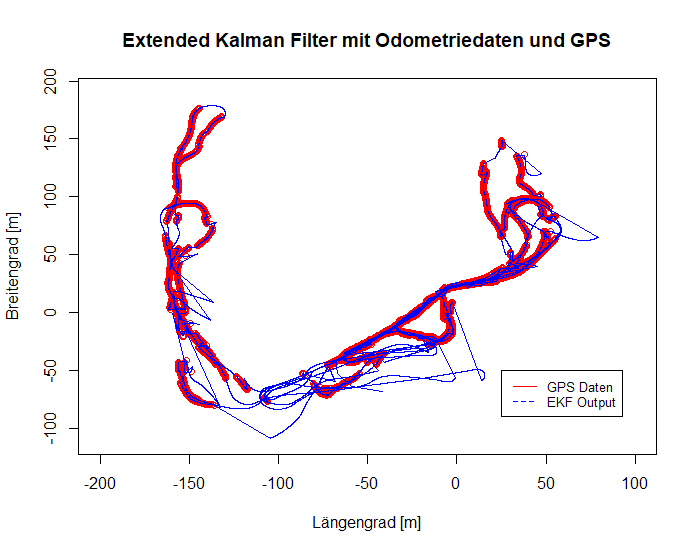
\includegraphics[width=5.5in]{EKF-output.png}
	\caption{Output des EKF mit GPS-Daten als Update.}
	\label{Flink-Überblick}
\end{figure}


\section{Zusammenfassung}\label{Zusammenfassung}

\section{Diskussion}\label{Diskussion}

\section{Appendix}\label{Appendix}


\bibliography{DBPro}
\bibliographystyle{ieeetr}

\end{document}
